% Use only LaTeX2e, calling the article.cls class and 12-point type.

\documentclass[11pt,twocolumn]{article}

\usepackage[utf8]{inputenc}
\usepackage{amssymb}
\usepackage{amsmath}
\usepackage{hyperref}
\usepackage{graphicx}

% Users of the {thebibliography} environment or BibTeX should use the
% scicite.sty package, downloadable from *Science* at
% www.sciencemag.org/about/authors/prep/TeX_help/ .
% This package should properly format in-text
% reference calls and reference-list numbers.

\usepackage{scicite}

% Use times if you have the font installed; otherwise, comment out the
% following line.

\usepackage{times}

% The preamble here sets up a lot of new/revised commands and
% environments.  It's annoying, but please do *not* try to strip these
% out into a separate .sty file (which could lead to the loss of some
% information when we convert the file to other formats).  Instead, keep
% them in the preamble of your main LaTeX source file.


% The following parameters seem to provide a reasonable page setup.

\topmargin 0.0cm
\oddsidemargin 0.2cm
\textwidth 16cm
\textheight 21cm
\footskip 1.0cm

\def\sectionautorefname{Section}
\def\tableautorefname{Table}
\def\figureautorefname{Figure}

% ACL style
\setlength\columnsep{0.6cm}


%The next command sets up an environment for the abstract to your paper.

\newenvironment{sciabstract}{%
\begin{quote} \bf}
{\end{quote}}

% The following lines set up an environment for the last note in the
% reference list, which commonly includes acknowledgments of funding,
% help, etc.  It's intended for users of BibTeX or the {thebibliography}
% environment.  Users who are hand-coding their references at the end
% using a list environment such as {enumerate} can simply add another
% item at the end, and it will be numbered automatically.

\newcounter{lastnote}
\newenvironment{scilastnote}{%
\setcounter{lastnote}{\value{enumiv}}%
\addtocounter{lastnote}{+1}%
\begin{list}%
{\arabic{lastnote}.}
{\setlength{\leftmargin}{.22in}}
{\setlength{\labelsep}{.5em}}}
{\end{list}}


% Include your paper's title here

\title{Dialog Management with Deep Neural Networks}


% Place the author information here.  Please hand-code the contact
% information and notecalls; do *not* use \footnote commands.  Let the
% author contact information appear immediately below the author names
% as shown.  We would also prefer that you don't change the type-size
% settings shown here.

\author
{Lukáš Žilka\\
\normalsize{zilka@ufal.mff.cuni.cz} \\
%\\
%\normalsize{Institute of Formal and Applied Linguistics,}\\
%\normalsize{Faculty of Matematics and Physics,}\\
%\normalsize{Charles University in Prague}\\
%\normalsize{Malostranske namesti 25, 118 00 Prague, Czech Republic}\\
}

% Include the date command, but leave its argument blank.

\date{}



%%%%%%%%%%%%%%%%% END OF PREAMBLE %%%%%%%%%%%%%%%%



\begin{document}

% Double-space the manuscript.

%\baselineskip24pt

% Make the title.

\maketitle

%\tableofcontents

%\newpage


\section{Introduction}

A dialog state tracker is an essential component of modern spoken dialog systems. It maintains the user's goals throughout the dialog by looking at the automatic speech recognition (ASR) results of her utterances. For example, in the restaurant information domain, the dialog state tracker tracks what kind of food the user wants and which price range is she looking for, and provides this information as a probability distribution over \emph{food} and \emph{price\_range}: $\operatorname{P(\mbox{food}, \mbox{price\_range})}$ The dialog state tracker also needs to deal with speech recognition errors and tries to reduce their impact on the dialog~\cite{williams2013dialog}.

The state-of-the-art dialog state trackers~\cite{williams2014web,henderson2014word,lee2014optimizing,smith2014comparative,sun2014sjtu} achieve their performance by learning from annotated data, and they were shown to work well in the restaurant information domain in the dialog state tracking challenge DSTC2~\cite{henderson2014second}. However, they possess several undesirable traits. First, they can only track the dialog state turn-by-turn (as opposed to a more complicated word-by-word approach), which limits the responsivity of the dialog system. Second, some of the trackers rely on the results from a spoken language understanding (SLU) component~\cite{wang2005spoken}, which brings an additional component into the dialog system that needs to be trained and tuned. Third, elaborate and complicated tracking models of the trackers are difficult to reproduce and maintain. In this thesis proposal we aim to address these problems.

The contribution of this thesis proposal is a novel approach to dialog state tracking.
It aims towards building more responsive and simpler dialog systems by proposing the first trainable dialog state tracker which naturally operates incrementally, word-by-word, and can directly learn from annotated dialogs, removing the need for an SLU unit. The word-by-word mode of tracking allows the dialog manager to be more responsive with the users. Simplicity comes from the fact that the whole dialog state tracker can be automatically optimized from data by a standard backpropagation algorithm, without requiring the user to manually tune opaque hyper-parameters or task-specific pre-processing.

Our approach is based on the modern deep learning techinques, particularly the long-short term memory recurrent neural network (LSTM RNN)~\cite{hochreiter1997long}.
We have chosen this approach due to several reasons:
First, LSTMs were shown to be effective for learning sequence mappings in automatic speech recognition~\cite{graves2005framewise}, machine translation~\cite{sutskever2014sequence}, protein structure prediction~\cite{sonderby2014protein}, and many other sequence classification tasks. The length of the sequences successfully modelled by LSTMs is comparable to the length to the word sequences in the spoken dialog systems.
Second, the sequential nature of the dialog naturally fits the LSTM's recurrent mode of operation. And finally, as the tracker processes the input, it incrementally builds an intermediate representation of the dialog. It has been shown that good intermediate representations help generalization~\cite{gulccehre2013knowledge}.
The success of LSTM on multiple complicated and diverse tasks promises to be exploitable also in dialog state tracking.

In the thesis proposal we explore several directions towards dialog state tracking with LSTM networks:
\begin{itemize}
  \item 1-best LSTM-based dialog state tracker
  \item n-best LSTM-based dialog state tracker
  \item Attention-based dialog state tracker.
  \item Reinforcement learning-based dialog state tracker.
\end{itemize}

The thesis proposal is organized as follows. First, we give an overview of the relevant spoken dialog systems and neural networks literature (\autoref{sec:soa}) and give a basic description of the task (\autoref{sec:dialog-state-tracking}). In \autoref{sec:lstm_dialog_state_tracker}, the model of the LSTM dialog state tracker is described with its training procedure. \autoref{sec:experiments} shows how it performs in the benchmarks. Finally, in \autoref{sec:discussion}, we discuss the results and qualities of the LSTM dialog state tracker, and conclude with \autoref{sec:conclusion}.


\section{Background}
This thesis builds upon the work from the fields of statistical spoken dialog systems and deep neural networks.

\subsection{Spoken Dialog Systems}
\label{sec:spoken_dialog_systems}
A spoken dialog system needs to understand what the user says, process it and provide an answer. Usually the dialog systems are turn-based, meaning that the system listens to the user and only replies when the user stops talking~\cite{thomson2010bayesian}. They are commonly built as a pipeline of several components:
\begin{enumerate}
  \item The automatic speech recognition (ASR) unit converts the user's speech to text.
  \item The spoken language understanding unit converts the text into structured information.
  \item The dialog management unit updates the dialog state and generates a system action.
  \item The structured system action is converted to natural text.
  \item The natural text is synthesized and spoken back to the user.
\end{enumerate}

\subsubsection{Automatic Speech Recognition}
Loosely speaking, the task of an automatic speech recognizer is to transcribe speech to text. More precisely, its task in the spoken dialog systems context is to decode the user's utterance into a structure called \emph{ASR hypothesis} that the next components of the system can use. Typically the hypothesis is either an 1-best list~\cite{gorin1997may,wang2003word}, an n-best list~\cite{he2003data}, a word confusion network\cite{hakkani2006beyond} or a word lattice~\cite{oerder1993word}. Word lattices are the richest but also the most complex structures to work with. It has been shown that using word lattices or word confusion networks in the spoken language understanding yields substantially better results over 1-best hypothesis~\cite{tur2002improving}.

There are open-source and commercial ASR solutions available with varying capabilities and purposes of use. The most pouplar open-source solution is Kaldi~\cite{povey2011kaldi}, which can be trained out-of-the-box to provide state-of-the-art ASR performance. Google Speech API\footnote{https://www.google.com/intl/en/chrome/demos/speech.html} is a popular commercial solution that is very fast and accurate for general speech and supports a lot of languages, but is not customizable and has unclear licensing conditions. Nuance's\footnote{http://dragonmobile.nuancemobiledeveloper.com/public/} commercial recognizers are more flexible but they are paid and closed-source. ISpeech ASR API\footnote{http://www.ispeech.org/api} is also customizable (users can select expected speech type: text messages, voice mail, dictation) but it does not allow full customization and is also paid. AT\&T Watson\footnote{http://developer.att.com/apis/speech} allows users to provide a custom grammar (language model) but
its free use is limited.

\subsubsection{Spoken Language Understanding}
Spoken language understanding (SLU) unit aims to interpret the user's intention from their speech utterance~\cite{wang2005spoken}. Particularly it converts the ASR hypothesis to its abstract meaning representation. For example ``yes'' could be transformed as ``affirm()'', or ``I want to go to Brno'' as ``inform(task=find\_connection)\&inform(to\_stop=Brno)'' in the meaning representation used in the ALEX dialog system~\cite{duvsek2014alex}. The meaning representation is arbitrary and adjusted to the particular dialog system. Examples of other representations can be found in~\cite{skantze2008galatea,he2003data}.

Historically, SLU has been done by manually writing grammars used to fill slots in semantic frames~\cite{ward1994recent,dowding1993gemini}, but this is expensive and non-flexible, because an expert needs to devise the grammar and then laborously maintain it. As the complexity of the domain grows the maintanence effort grows much more. Instead, statistical approach to SLU has been adopted, where SLU is viewed as a pattern recognition problem
$$\hat M=\operatorname{arg~max}_M \operatorname{P}(M|W)$$
where we are looking for the best abstract meaning representation $M$ of the input given the ASR hypothesis $W$. The main benefit of this approach is the ability of the model to leverage the training data to improve its performance. HMM can be used to model the joint probability of the words and abstract meaning representation given the acoustic signal~\cite{pieraccini1992progress,pieraccini1992stochastic}. Hidden Vector State model that learns stack operations to parse the user's utterance in a hierarchical way was proposed~\cite{he2003data}. It is particularly appealing for its ability to infer the hierarchy in the user's utterances without explicit hierarchical annotations. Markov Logic Networks were used for SLU by~\cite{meza2008spoken}, where first-order logic formulaes are used as templates to instantiate complex Markov network that model the slot-value representation. In~\cite{zettlemoyer2007online} an algorithm that learns to parse the text input into lambda-calculus expressions using extended combinatory categorial grammar is given.

\subsubsection{Dialog Management}
Dialog management component directly influences how natural and intelligent will the dialog system be perceived among its users. Its task is to come up with the next action of the system given the previous progress of the dialog. It usually consists of two parts: dialog state tracking, and dialog action selection.

Dialog state tracking watches the dialog progress and keeps track of important information in form of the dialog state, or as a probability distribution over all possible dialog states called the belief state. The dialog state is a structure that contains several components that take several values, for example a component ``food'' that can take values ``chinese'', ``indian'', or ``thai'', and a component ``area'' that take values ``north'' and ``south'', and usually only the information needed for the dialog action selection is tracked.

Dialog action selection acts upon the dialog state or the belief state to generate the next action. There are handcrafted approaches to the next action selection~\cite{pieraccini2005we,skantze2008galatea}, and approaches that automatically learn from observing rewards~\cite{levin2000stochastic,walker2000application,lemon2006isu,thomson2010bayesian}.

\paragraph*{Bayesian Networks}
Bayesian networks can be used for the belief state tracking~\cite{pulman1996conversational,williams2007applying,bui2006tractable,thomson2010bayesian}. The belief $b$ is updated as
$$b'(s)=\frac{1}{Z} \cdot P(o'|s,a)\sum_{s'}P(s|s',a)b(s')$$
where $o$ is the observation, typically the user utterance, $s$ is the dialog state and $a$ is the system action.

\paragraph*{Recurrent Neural Network Tracker}
Using recurrent neural network (RNN) for dialog state tracking has been proposed in~\cite{henderson2014word,henderson2013deep} using n-grams from n-best lists as features.

\paragraph*{Ranking-based Tracking}
The dialog state tracking was poisted as a ranking problem in~\cite{williams2014web}, where all the possible dialog states given the observed SLU hypotheses are enumerated and then ranked using a LambdaMART ranking algorithm.

\paragraph*{Discriminative Model Tracking}
Generalized linear regression model $f$ was trained to update the belief state
$$b'(s)=f(b(s), a, o)$$
and shown to outperfrom heuristic upddate rules~\cite{bohus2006k}.

\subsubsection{Natural Language Generation}
The natural language generation (NLG) component generates the natural language utterance of the system action. For example, if the system generates the action \texttt{confirm(food=chinese)} then the NLG should generate ``Did you say chinese food?''. The simplest approach is a template-based NLG that has a database of templates, where for each possible system action there is a template to be used~\cite{duvsek2014alex}. More sophisticated approach is a data-driven model that given a corpus of (system action; its surface realization) pairs learns to generate the natural language utterances~\cite{mairesse2010phrase}.

\subsubsection{Speech Synthesis}
Speech synthesis takes the natural language utterance generated by NLG and transforms it to speech signal. Two main approaches are used: 1.) concatenative speech synthesis~\cite{campbell1997prosody,masuko1996speech}, and 2.) statistical parametric speech synthesis~\cite{zen2009statistical}

The concatenative speech synthesis (also called unit-selection synthesis) uses a database of speech segments, from which it selects some of them, and concatenates them together to form the speech signal. For each speech unit to be synthesized it tries to find the most appropriate segment in terms of the similarity to the sound to be synthesized and the smoothness of concatenation with other segments.

Statistical parametric speech synthesis directly models the acoustics of the speech. During the training of the model, linguistic $l$ and acoustic features $a$ are extracted from the training data and a conditional model of $p(a|l)$ found. During synthesis the best acoustic features for the given linguistics features are found $\hat{a}=\operatorname{arg~max}_a p(a|l)$. HMM\cite{yoshimuray1999simultaneous}, DNN~\cite{ze2013statistical}, and RNN~\cite{zen2015unidirectional} were used as the conditional models.

\section{LSTM Dialog State Tracker}
\label{sec:dialog-state-tracking}
The task of dialog state tracking is to monitor progress in the dialog and provide a compact representation of the dialog history in the form of a \emph{dialog state}~\cite{henderson2014second,zilka2013comparison}. Because of uncertainty in the user input, statistical dialog trackers maintain a probability distribution over all dialog states, called the \emph{belief state}. As the dialog progresses, the dialog state tracker updates this distribution given new observations.

In this paper, we define the dialog state at time $t$ as a vector $s_t \in C_1 \times ... \times C_k$ of $k$ dialog state components, sometimes called slots in the literature. Each component $c_i \in C_i=\{v_1, ..., v_{n_i}\}$ takes one of the $n_i$ values. Our dialog state tracker maintains a probability distribution over $s_t$ factorized by the dialog state components:
$$P(s_t|w_1, ..., w_t)=\prod_i p(c_i|w_1, ..., w_t; \theta)$$

Note that all models $p(c_i|\cdot)$ share a substantial portion of the parameters, as detailed in the next section, so despite the fact that the predictions are factorized and thus independent, they were optimized to minimize a joint objective function and therefore naturally model the dependence between the dialog state components.




\subsection{Deep Neural Networks}
Neural networks is an old field

The progress in computational power made neural networks feasible.



LSTM Dialog State Tracker
LSTM Dialog State Tracker with Knowledge Graph
Attention-based Dialog State Tracker
Reinforcement learning-based Dialog State Tracking

\section{LSTM-based Dialog State Tracker}
Our model fits in the big picture of a spoken dialog system described in~\autoref{sec:spoken_dialog_systems} as a dialog state tracker in the dialog management unit. Also it removes the need for the spoken language understanding unit, thus connects straight to the automatic speech recognition results.

\section{LSTM Dialog State Tracker}
\label{sec:lstm_dialog_state_tracker}
Here we define our novel LSTM dialog state tracking model. Its task is to map a sequence of words in the dialog $w_1$, ..., $w_t$ to predictions for each of the $k$ dialog state components $(p^{(1)}_t, ..., p^{(k)}_t)$. Each $p^{(i)}_t$ is a vector corresponding to a probability distribution over the values of the i-th dialog state component. For example, $p^{(area)}_t$ is a probability distribution over values $\{north, south, east, west\}$ at the time $t$.

\begin{figure*}
\center
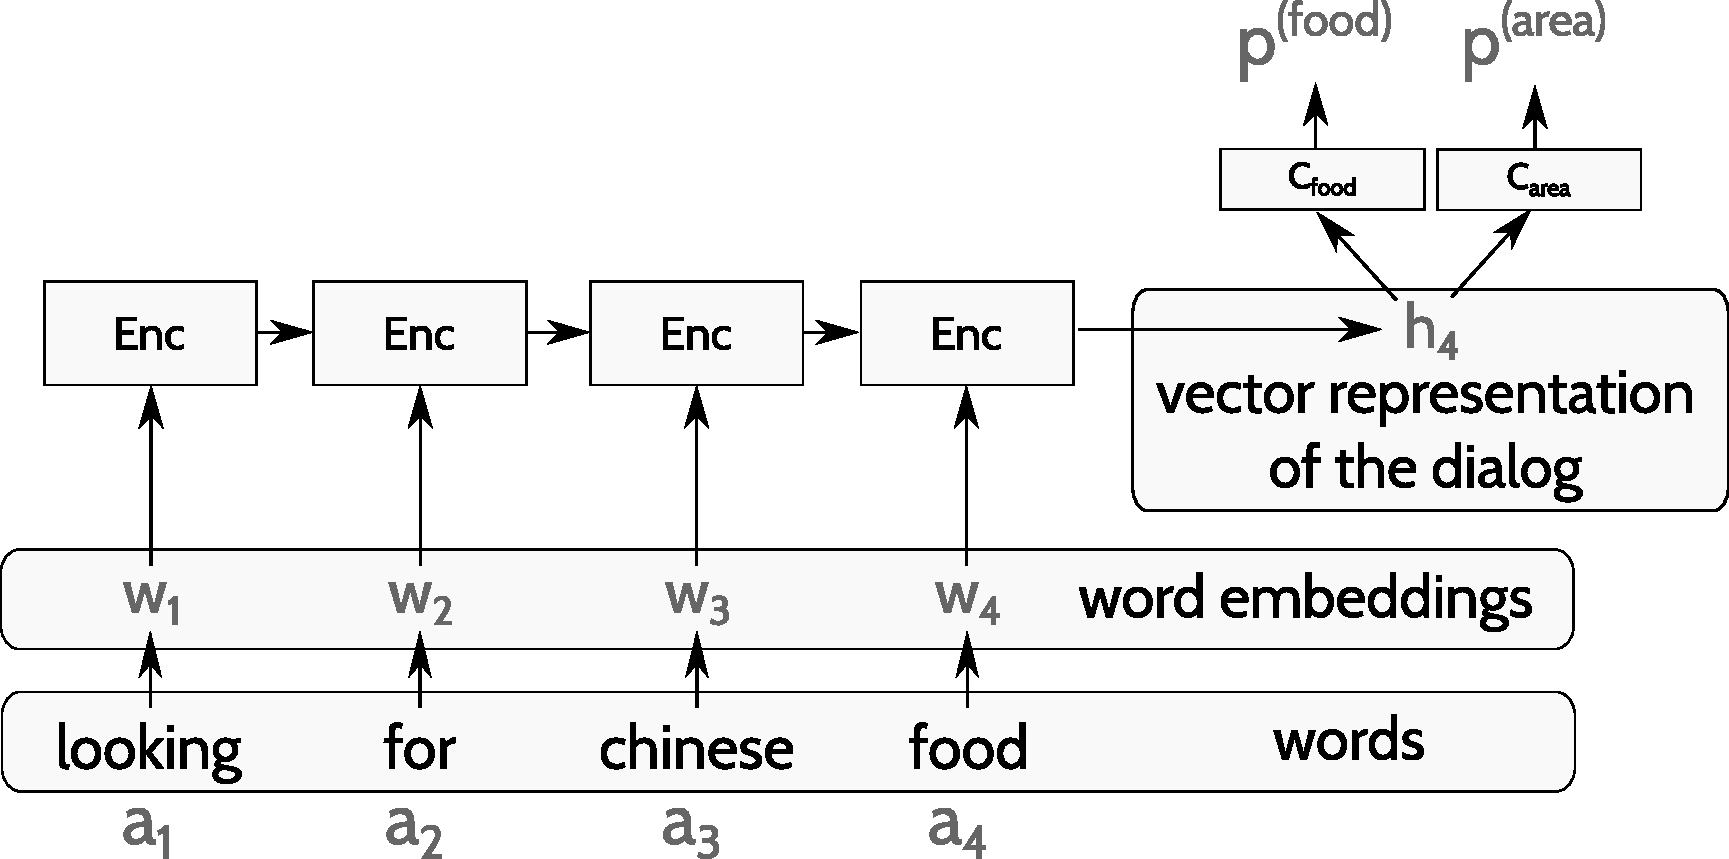
\includegraphics[width=0.75\textwidth]{arch}
\caption{A demonstration of the LSTM Dialog State Tracker applied to a user utterance ``looking for chinese food''. The encoding LSTM model $Enc$ is sequentially applied to each input word and at the end, its hidden state is used to feed to the state component classifiers.}
\label{fig:LecTrack}
\end{figure*}

\subsection{Model}
Our dialog state tracking model can be seen as an encoder-classifier model, where an LSTM is used to encode the information from the input word sequence into a fixed-length vector representation. Given this representation, the classifier predicts a value for each of the dialog state components (as a probability distribution).

Formally we have an encoder that maps an input word and a previous hidden state to a new hidden state, $Enc(w, h_{t-1})=h_t$, and a classifier that maps a hidden state to a prediction, $C(h_t)=p_t$. To encode the whole dialog, the encoder is applied sequentially on the input sequence of words. In our system, we have one encoder $Enc$ and multiple classifiers $C$, one for each dialog state component (e.g. $C^{(food)}$, $C^{(area)}$, ...).

%\subsection{Notation}  % TODO: Maybe put as a footnote.
%We use capital letters to denote matrices, lower-case letters to denote vectors and scalars, and $\odot$ is an element-wise product of vectors. $\sigma$ denotes the logistic function $\sigma(x) = \frac{1}{1+e^{-x}}$, $\operatorname{ReLU}(x)=max(0, x)$ is the rectified linear unit, and $\operatorname{softmax}(x)=\frac{e^x}{\sum_i e^{x_i}}$.

\subsection{Tracker Model}
The LecTrack tracker is composed of two major components: the encoder $Enc$ and the classifier $C$.

The model of the encoder $Enc$ is a LSTM RNN~\cite{hochreiter1997long,zaremba2014recurrent}, parametrized by $W_{(enc)}$ and $b_{(enc)}$:
\begin{align*}
\bf{Enc}: & w_t, (h_{t-1}; c_{t-1}) \rightarrow  (h_t; c_t) \\
\begin{pmatrix}
i_t \\
f_t \\
o_t \\
g_t
\end{pmatrix} &=
\begin{matrix}
\sigma \\
\sigma \\
\sigma \\
tanh
\end{matrix}
[
W_{(enc)}
\begin{pmatrix}
x_t \\
h_{t-1}
\end{pmatrix}
+
b_{(enc)}
] \\
c_t &= f_t \odot c_{t-1} + i_t \odot g_t \\
h_t &= o_t tanh(c_t)
\end{align*}

The vectors $i_t, f_t, o_t, g_t$ represent the input, forget, output and modulation gates, respectivelly, the vector $c_t$ is the cell state and the vector $h_t$ denotes the output, following the standard LSTM literature~\cite{hochreiter1997long,zaremba2014recurrent}.
In case of a recursive application of $Enc$, we write $Enc(w_1, ..., w_n, h, c)$ instead of $Enc(w_n, ... Enc(w_1, h, c))$ to simplify the notation.

The model of the classifier $C$ is a neural network with a single layer composed of rectified linear units and a softmax output layer:
\begin{align*}
\bf{C}: & h_t \rightarrow p_t \\
p_t &= \operatorname{softmax}(W_p \cdot \operatorname{ReLU}(W_h h_t + b_h) + b_p) \\
\end{align*}

The encoder and classifier form together the LecTrack LSTM dialog state tracker:
\begin{align*}
\bf{LecTrack}: & ~a_1, ..., a_n \rightarrow p_{1}, ..., p_{k} \\
\forall i \in {1, ..., k}: & ~p_i = \operatorname{C_i}(\operatorname{Enc}(E \cdot a_1, ..., E \cdot a_n, h_0, c_0))
\end{align*}
Here, $n$ is the length of the input sequence, $k$ the number of the dialog state components, $a_1$, ..., $a_n$ is the input word sequence encoded in a one-hot encoding, $E$ is a word embedding matrix, and $h_0=c_0=\bf{0}$ are zero vectors. As shown, each token $a_i$ is mapped to its corresponding embedding vector through the embedding matrix $E$, $w_i=E\cdot a_i$. The literature suggests many ways for obtaining the embedding matrix $E$~\cite{mikolov2013efficient,kim2014convolutional,stratosspectral}, but in the experiments in this paper, we treat it just as another set of parameters for the sake of simplicity.\footnote{Informal experiments with different types of initialisaion of word embedings, such as using word2vec~\cite{mikolov2013efficient} embedings estimated from a large out-of-domain corpus, did not suggest any advantage over randomly initialised embeddings in this relatively limited domain. Therefore, we decided not to explore this direction further.}

\subsection{Training}
The model is trained using the standard cross-entropy criterion~\cite{rubinstein2004cross} in the vanilla stochastic gradient descent scenario~\cite{bottou2010large}:
$$ l(a_1, ..., a_n, y_1, ..., y_k; \theta) = \sum_{i=0}^k \operatorname{log} \operatorname{LecTrack}(a_1, ..., a_n)^i_{y_i}$$
Here, $\operatorname{LecTrack}(.)^m_n$ denotes the probability of the $n$-th value in the $m$-th dialog state component.

After each optimization epoch, we monitor the performance~\footnote{See the experiments section for the description of the featured metrics.} of the model on a held-out set $D$. When the performance stops increasing for several iterations, we terminate the training and select the best-performing model.


\section{Experiments}
\label{sec:experiments}
\subsection{Dataset}
To train and evaluate our model, we use the DSTC2~\cite{henderson2014second} data, which is a common data set for dialog state tracking evaluation. The DSTC2 data consists of about 3,000 dialogs from the restaurant information domain, each dialog is 10 turns long on average. The data is split into training, development and test sets. This data allows us to measure the performance of our tracker on turn-based dialogs. Ideally we would run the evaluation on a dataset where we could also measure the incremental capabilities of the tracker, but to the best of our knowledge, no such dataset is publicly available yet, and we shall address this in our future work.

\subsection{Baseline}
A baseline system for this domain has been provided by the DSTC2 organizers. It uses the SLU results and confidence to rank hypotheses for the values of the individual dialog state components. There were several baselines described in~\cite{henderson2014second} and we report the results of the \emph{focus} baseline, which was the best among them.

\subsection{Data Preprocessing}
Each dialog turn contains the system utterance and the user utterances, which we need to serialize into a stream of words as the input to our model. The system utterance undergoes a simple preprocessing detailed below, and the user utterance is directly fed to the model word-by-word without any further preprocessing. There is no difference between the system and user utterance in the eyes of our model, both are seen together as one long sequence of words.

\subsubsection{System Input:}
To get the the system input, we perform a simple preprocessing. We flatten the system dialog acts of the form \texttt{act\_type(slot\_name=slot\_value)} into a sequence of two tokens $t_1, t_2$, where $t_1=(\operatorname{act\_type}, \operatorname{slot\_name})$ and $t_2=\operatorname{slot\_value}$. For example \texttt{request(slot=food)} is flattened as $(request, slot), food$, which the model then sees as a word sequence of length two\footnote{The whole system sentences could be used and result in a similar performance under the measured metrics, but also increase the training time of the model and contain no more information than the stringified dialog acts. Therefore, we only use the flattened dialog acts.}. The resulting tokens are added to the vocabulary of the model side by side with the words from the user utterances, but in such a way that they are still differentiated from the user's words of the same form. For example, the system act \texttt{inform(food=chinese)} results in the tokens \texttt{(inform, food)} and \texttt{chinese}. But the user utterances also contain the word \texttt{chinese}, so if we put both the system tokens and the user words into one vocabulary, they would be mixed. We care to keep them separate because we empirically found that mixing user words and system tokens to be harmful to the performance of the tracker.

\subsubsection{User Input:}
For the sake of simplicity, we use only the best live-ASR\footnote{There are batch and live ASR results in the DSTC2 data. We use the live ones and refer to them as live-ASR.} hypothesis and ignore the rest of the n-best list.
We plan to extend our model for processing multiple ASR hypotheses in the near future.
%Therefore, we leave the more involved extensions of our model capable of processing the whole n-best list for future work.

\subsubsection{Out-of-Vocabulary Words}
are randomly mixed into the training data to give the model a chance to cope with unseen words: At training time, a word in the user input word is replaced by a special out-of-vocabulary token with probability $\alpha$. At test time, this token is used for all unknown words.

\subsection{Experimental Methodology}  % TODO: Prilis strucne.
We follow the DSTC2 methodology~\cite{henderson2014second} and measure the accuracy and L2 norm of the joint slot predictions.
The joint predictions are grouped into the following groups, and the results of each group is reported separately: Goals, Requested, Method.
%Goals (each 5-75 values): area, food, name, pricerange; 2.) Requested (each a binary decision): request\_address, request\_area, request\_food, request\_name, request\_phone, request\_pricerange; 3.) Method (5 values): method
For each dialog state component in each dialog the measurements are taken \emph{at the end of each dialog turn}, provided the component has already been mentioned in some of the SLU n-best lists in the dialog\footnote{Note we do not use the SLU n-best list in our model at all, but we adapt this metric to be able to compare to the other trackers in DSTC2.}

%\subsection{Implementation Details}
%We used the Theano~\cite{bastien2012theano} deep learning framework to implement our model. During model training, we use the dropout technique~\cite{hinton2012improving} and the following values of learning parameters, chosen based on several rounds of manual grid search:
%\begin{itemize}
%    \item learning rate = 0.1
%    \item batch size = 1
%    \item number of LSTM neurons = 80
%    \item number of output hidden neurons = 96
%    \item dropout rate = 0.5
%    \item embedding size = 80
%    \item gradient clipping = 5
%    \item initial bias of forget gates = 40
%\end{itemize}
%Typically it takes around 500 epochs, which is roughly 24 hours, to find the best model on a single-CPU 2GHz Xeon 5130 machine.

\subsection{Results}
The results of LecTrack on the DSTC2 data are summarized in~\autoref{table:results}. For the groups \emph{Method} and \emph{Requested} LecTrack's accuracy is better than the baseline and comes closer to the state-of-the-art. Within these groups the handcrafted preprocessing present in the baseline and the state-of-the-art models is not as effective as for the \emph{Goal} group.

We hypothesize that the accuracy on the \emph{Goal} group does not achieve the state of the art because of two reasons. First, LecTrack needs to see examples for each value of each dialog state component. But the distribution of the individual values in the data has a heavy tail, and thus the baseline method and state-of-the-art methods that use various kinds of handcrafted abstraction to make the data denser and leverage hand-crafted generalization beat LecTrack. Second, our model does not utilize the information in the n-best lists, thus loses useful information in the uncertain cases where more hypotheses than the first one are useful.

For the frequently seen values from the group \emph{Goal} the performance of LecTrack is much better than the baseline, as is shown in~\autoref{table:resultsFreq}. We looked at the sub-goal \emph{food} and compared the classification accuracy of its individual values. The top of the table contains 9 values, which occur more than 100 times in the test set, as the representatives of the classes that are well-represented in the data; the bottom of the table contains the representatives of the under-represented classes, and we selected values which occur at least 10 times in the test set to get meaningful accuracy estimates. For the well-represented classes, LecTrack's performance is stable and usually beats the baseline by a large margin, however for the under-represented classes LecTrack's performance is much worse than the baseline. This suggests that some form of abstraction should improve the results for the under-represented cases.

To keep the model simple we did not use any form abstraction, such as gazeteers to preprocess our data, and only used 1-best hypothesis as an input. Gazeteers offer a cheap solution to data sparsity for English but are difficult to gather and maintain for other languages where one word can have many forms. In our future experiments we plan to introduce some form of abstraction. Also, it is not obvious from the machine learning literature how an n-best list could be used in the model to improve the performance. This is another aspect that will be addressed in our future experiments.

\begin{table*}
    \centering
    \begin{tabular}{|c|llllll|llllll|}
    \hline
    & \multicolumn{6}{c|}{Dev}                                                                & \multicolumn{6}{c|}{Test}  \\
     & \multicolumn{2}{c}{Goal} & \multicolumn{2}{c}{Method} & \multicolumn{2}{c|}{Requested}  & \multicolumn{2}{c}{Goal} & \multicolumn{2}{c}{Method} & \multicolumn{2}{c|}{Requested} \\
    model                          & Acc.    & L2      & Acc.   & L2      & Acc.    & L2     & Acc.    & L2      & Acc.    & L2     & Acc.     & L2 \\ \hline \hline
    baseline                       & 0.61      & \bf{0.63} & 0.83      & 0.27      & 0.89      & 0.17      & 0.72      & 0.46      & 0.90      & 0.16      & 0.88      & 0.20    \\
    LecTrack                         & 0.62      & 0.79      & 0.87    & 0.24 &  0.95  &  0.09     & 0.60      & 0.79      & 0.91      & 0.17  & 0.96 & 0.07    \\

    \cite{williams2014web}\footnote{state-of-the-art}         & \bf{0.71} & 0.74      & \bf{0.91}      & \bf{0.13}      & \bf{0.97} & \bf{0.05}      & \bf{0.78} & \bf{0.35} & \bf{0.95}  & \bf{0.08}      & \bf{0.98} & \bf{0.04}   \\ \hline
    \end{tabular}
    \medskip
    \caption{Performance on the DSTC2 data.}
    \label{table:results}
\end{table*}

\begin{table}
    \centering
    \begin{tabular}{|r|ll|}
    \hline
               value & baseline & LecTrack \\
    \hline
             chinese   & 0.53   & 0.82   \\
              indian   & 0.49   & 0.79   \\
              korean   & 0.67   & 0.93   \\
      asian oriental   & 0.54   & 0.86   \\
            dontcare   & 0.98   & 0.88   \\
            european   & 0.61   & 0.80   \\
             italian   & 0.41   & 0.79   \\
             spanish   & 0.69   & 0.73   \\
                thai   & 0.14   & 0.64   \\
    \multicolumn{3}{|c|}{...} \\
                traditinal  & 0.17  & 0.17 \\
               steakhouse   & 0.14  & 0.07 \\
                romanian    & 0.35  & 0.21 \\
                german      & 0.28  & 0.07 \\
    \hline
    \end{tabular}

    \medskip
    \caption{Accuracy for the most frequent values for the \emph{food} dialog state component which have at least 100 test examples in the test set, and for some that contain between 10 to 20 examples in the test set.}
    \label{table:resultsFreq}
\end{table}

\section{Discussion}
\label{sec:discussion}
Our LSTM dialog state tracker is capable of learning from raw dialog text, annotated with true dialog state component values at some timesteps. No spoken language understanding unit is needed to pre-process the input for our model. In addition, the model performance does not suffer if the input word sequences are long, which is in accordance with other LSTM applications~\cite{sutskever2014sequence}.

Our model naturally handles the inter-slot dependence by projecting the input sequence into a fixed-length vector from which all the dialog state component predictions are made. However, the predictions are made independently for all of the state components and the joint distribution is not explicitly modelled.

Provided the ASR decodes also non-speech events, e.g., the affirmative "hmm" or "oh" or the information that the user is silent, the model can naturally learn to interpret them and provide hints to the dialog manager, such as whether the user seems to be confused, or if they started saying something and the dialog manager should interrupt its speech production and listen instead. In noisy conditions, waiting for silence is very limiting for the dialog system. The tracker's ability to process the input incrementally can overcome this issue and signal to the dialog manager when the incoming speech starts to make sense. This can lead to more human-like and interactive dialogs and simpler dialog managers. Our model was designed to be able to predict at arbitrary time in the dialog the full distribution over the dialog state components, and this mode of operation costs no additional computation as opposed to other trackers.

\section{Related Work}
\label{sec:related}

The only incremental dialog system in the literature that we are aware of is~\cite{skantze2009incremental}. In this paper, the authors describe an incremental dialog system for number dictation as a specific instance of their incremental dialog processing framework \cite{schlangen2009general}. To track the dialog state, they use a discourse modelling system~\cite{skantze2008galatea}, which keeps track of the confidence scores from the semantic parses of the input. The semantic parses are produced by a grammar-based semantic interpreter~\cite{skantze2004robust} with a hand-coded context-free grammar. While their system is mostly handcrafted, ours is trained using annotated dialog data, so we do not need the handcrafted grammar and an explicit semantic representation of the input.

Using RNN for dialog state tracking has been proposed before~\cite{henderson2014word,henderson2013deep}. The dialog state tracker in~\cite{henderson2014word} uses an RNN, with a very elaborate architecture, to track the dialog state turn-by-turn. Similarly to our model, their model does not need an explicit semantic representation of the input. However, unlike our model, they use tagged n-gram features, which allows them to perform better generalization on rare but well-recognized values. Our model is capable of such generalization, too, but it needs more data. We refrain from using the tagged features because they introduce a preprocessing effort, and we are interested in a model that can learn from the data directly without assuming any correspondence between the names and values of the dialog state components and their surface forms that occur in the dialog (e.g. that value ``chinese'' of the dialog state component ``food'' will typically be represented as ``chinese food'' in the dialog). In English dialog systems, it might be perceived as an unneccessary complication not to leverage these tagged features, but when we consider other languages, where a word often has a lot of forms, it pays off, because the effort spent on producing quality tagged features is non-trivial.


\section{Conclusion}
\label{sec:conclusion}
We presented a first trainable incremental dialog state tracker that directly uses automatic speech recognition hypotheses to track the state. It is based on a long short-term memory recurrent neural network and fully trainable from the dialog utterances annotated at certain points in time by the dialog state information. It represents the history of the whole dialog as a low-dimensional real vector, which is on its own used for the prediction of the whole dialog state. We evaluated our dialog state tracker on the data from Dialog State Tracking Challenge 2, where we showed that it achieves a promissing performance on the \emph{Method} and \emph{Requested} tracking sub-tasks. We believe that the simplicity, ease of use, and the incremental tracking capability of LecTrack make it a first good step on the way towards more responsive dialog systems.




\section{Future Work}
%  Neural reinforcement learning. Attention-based models.
%  Knowledge base tracking.


\section{Summary and Work Plan}


\bibliography{scibib}

\bibliographystyle{apalike}

\end{document}




















